\newpage
\hypertarget{rules vis}{}
\subsection{Visual TGG Rules}
\visHeader

EA distinguishes the different elements of a TGG rule with distinct visual and spatial clues. Correspondence elements, for example, are depicted as
hexagonal boxes, while attribute constraints are depicted as notes, referencing the relevant object variables.

\subsection{BoxToDictionaryRule}

\begin{enumerate}

\item[$\blacktriangleright$] In EA, open the \texttt{Rules} diagram of your TGG project we pointed out earlier. Create your first rule by either hitting the
\texttt{spacebar} and selecting \texttt{Rule} from the context menu, or performing a drag-and-drop of the \texttt{Rule} item from the TGG toolbox to the left of
the diagram window (Fig.~\ref{ea:create_tgg_rule}). Press \texttt{Alt + Enter} to raise its \texttt{Properties} dialogue, and update its name to
\texttt{BoxToDictionaryRule}.

\vspace{0.5cm}

\begin{figure}[htbp]
\begin{center}
  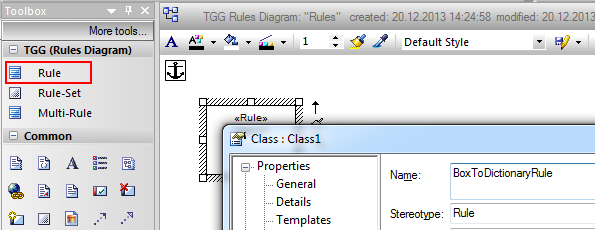
\includegraphics[width=\textwidth]{ea_TGGNewRule}
  \caption{Creating a TGG rule}
  \label{ea:create_tgg_rule}
\end{center}
\end{figure}

\vspace{0.5cm}

\item[$\blacktriangleright$] Double-click the element to open its rule diagram. Drag-and-drop \texttt{Box} from the project browser into the diagram once
again, choosing to paste the element as an \texttt{instance}.\footnote{If the `Paste Element' dialogue doesn't appear, hold \texttt{Ctrl} while dragging and
dropping and confirm you haven't selected the autosave option under \texttt{options}.} The \texttt{name} and \texttt{binding operator} should already be set to
\texttt{box} and \texttt{create}. Repeat the action to create an instance of \texttt{Dictionary}.

\newpage

\item[$\blacktriangleright$] Quick-link from \texttt{box} to \texttt{dictionary} this time to create a TGG correspondence \emph{link}. To keep things simple and
self-explanatory, keep the default name \texttt{boxToDictionary} and select the \texttt{BoxToDictionary} correspondence type from the drop-down list (which you
declared in the schema).

\vspace{0.25cm}

Believe it or not, with just this link, our rule \emph{already} creates a \texttt{Box}, \texttt{Dictionary}, and correspondence link between them at the same
time! Unfortunately, this only creates the objects, and doesn't relate any of their attributes. Why don't we try to connect the \texttt{name} of the
\texttt{box} to the \texttt{title} of the dictionary so that they always match?

\vspace{0.25cm}

For this, we use \emph{attribute constraints}.\footnote{First defined in Part III, Section 4} When used in TGG rules, attribute constraints provide a
bidirectional and high-level solution for attribute manipulation. In this case, we want to ensure that \texttt{box.name} and \texttt{dictionary.title} remain
consistent.

\vspace{0.5cm}

\item[$\blacktriangleright$] Following a similar process as creating a new \texttt{Rule}, either hit the \texttt{spacebar} or use the toolbox to create a
\texttt{TGG Constraint} (Fig.~\ref{ea:common_toolbox}).  Double-click the empty note to open its \texttt{TGGConstraint Dialog}.

\vspace{0.5cm}

\begin{figure}[htbp]
\begin{center}
  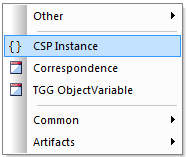
\includegraphics[width=0.3\textwidth]{ea_createTGGConstraint}
  \caption{TGG constraint from the toolbox}
  \label{ea:common_toolbox}
\end{center}
\end{figure}

\item[$\blacktriangleright$] You'll notice a pre-populated list of available constraints. Choose \texttt{eq} (representing `equals') and double-click each of
the \texttt{Value} fields to specify the \texttt{a} and \texttt{b} values as depicted in Fig.~\ref{ea:first_tgg_constraint}. Press \texttt{Add} to save the
constraint, then \texttt{OK} to affirm and close the window.

\item[$\blacktriangleright$] Your rule should now resemble Fig.~\ref{ea:tgg_rule_with_constraint}, where the new arrows indicate the constraint dependencies.

\newpage

\begin{figure}[htbp]
\begin{center}
  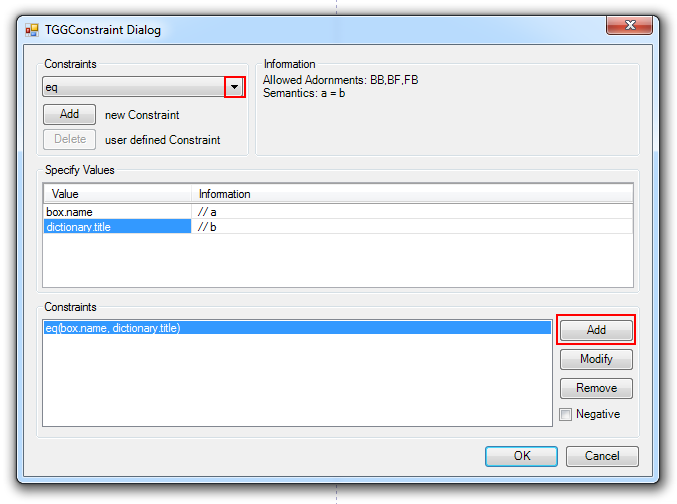
\includegraphics[width=\textwidth]{ea_TGGConstraintDialog}
  \caption{Completing the constraint}
  \label{ea:first_tgg_constraint}
\end{center}
\end{figure}

\vspace{1cm}

\begin{figure}[h!]
\begin{center}
  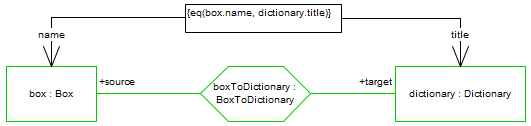
\includegraphics[width=0.9\textwidth]{ea_BoxToDictionaryRuleConstraint}
  \caption{A TGG rule with an attribute constraint}
  \label{ea:tgg_rule_with_constraint}
  \end{center}
\end{figure}

\newpage

Our first TGG rule is not yet complete. Our goal is to transform a \texttt{Box} into a \texttt{Dictionary}, so we still need to create the initial
structure of the learning box. In contrast to the rather simple dictionary, where \texttt{Dictionary} is a direct container for every \texttt{Entry} object, we
have to create a number of connected \texttt{Partitions} to hold the \texttt{Cards}.

\vspace{0.5cm}

\item[$\blacktriangleright$] Given that there are three valid difficulty levels for every \texttt{Entry} we create three \texttt{Partition} object variables,
complete with appropriate link variables that satisfy the Leitner's Box rules (the \texttt{next}, \texttt{previous}, and \texttt{box} references). Your TGG rule
should come to resemble Fig.~\ref{ea:boxtodictionaryrule_complete}.\footnote{To review how to set object attribute constraints, review Part III, Section 4}

\vspace{0.5cm}

\begin{figure}[htbp]
\begin{center}
  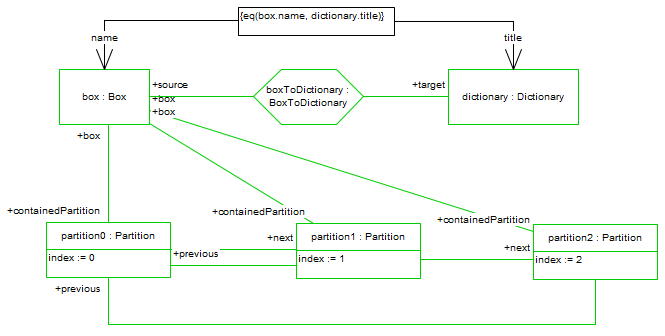
\includegraphics[width=\textwidth]{ea_BoxToDictionaryRuleComplete}
  \caption{Complete TGG rule diagram for \texttt{BoxToDictionaryRule}}
  \label{ea:boxtodictionaryrule_complete}
  \end{center}
\end{figure}

\end{enumerate}

Fantastic work! The rule of our transformation is complete! If you are in hurry, you can jump ahead and proceed to Section~\ref{sect:TGGs_in_Action}:
TGGs in Action. There you can transform a box to a dictionary and vice-versa, but please be aware that your specified TGG (with just one rule) will only be able
to cope with completely empty boxes and dictionaries. Handling additional elements (i.e., cards in the learning box and entries in the dictionary) requires a
second rule. We intend to specify this next.

% --------------- Card To Entry ------------------------------------------------------------------------------------------------------------------------
\clearpage
\subsection{CardToEntryRule}

The next goal is to be able to handle \texttt{card} and \texttt{entry} elements. The challenge is that it will require a strict pre-condition -- you should not
be able to transform these child elements unless certain structural conditions are met. In other words, we need a rule that demands an already existing
\texttt{box}, \texttt{dictionary}, and \texttt{partition}. It will need to combine `black' and `green' variables! Luckily, eMoflon has a cool feature
in its visual syntax to help with this. We can go to any existing rule and \emph{derive} a new one from it. The benefits of this may not be so obvious with this
small example, but this could potentially be a real time-saver in a large project.

\begin{enumerate}
  
\item[$\blacktriangleright$] First confirm that your eMoflon control panel window is open in the \texttt{Box\-To\-Dictionary\-Rule} diagram. Then hold
\texttt{Ctrl} and select \texttt{box}, \texttt{box\-To\-Dictionary},
\texttt{dictionary} and \texttt{partition0} simultaneously.
  
\item[$\blacktriangleright$] Switch to the \texttt{eMoflon TGG Functions} tab on the control panel and press \texttt{Derive} (
Fig.~\ref{ea:derive_from_tgg_rule}). In the dialogue that appears, enter \texttt{Card\-To\-Ent\-ry\-Rule} as the name of the rule, and press \texttt{OK.} The
new rule will automatically open in a new window.

\begin{figure}[htbp]
\begin{center}
 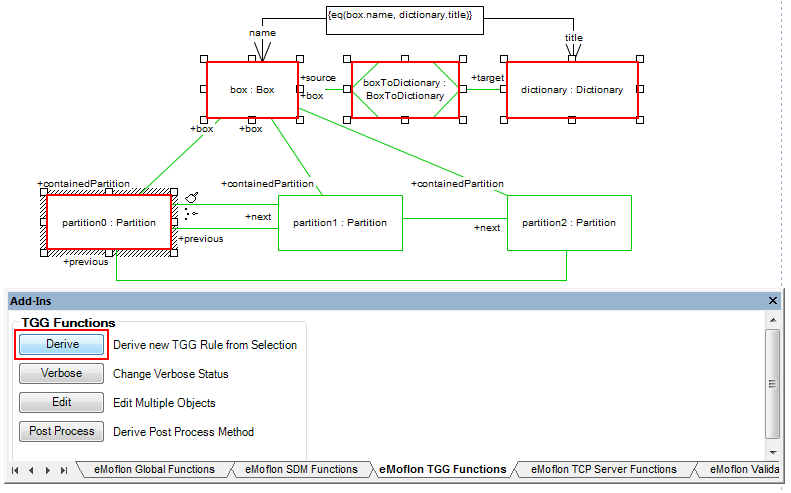
\includegraphics[width=0.7\textwidth]{ea_deriveCardToEntry}
  \caption{Derive a new rule from an existing one}
  \label{ea:derive_from_tgg_rule}
\end{center}
\end{figure}
\FloatBarrier

\item[$\blacktriangleright$] Add green instances of \texttt{Card} and \texttt{Entry} to the new rule, and link them to their respective \texttt{partition0} and
\texttt{dictionary} elements. 

\vspace{0.5cm}

\item[$\blacktriangleright$] Quick-link from \texttt{card} to \texttt{entry} and create another TGG correspondence link. You'll notice that the
\texttt{select correspondence link} drop-down menu is empty -- we haven't defined one between these types yet in the schema. Luckily, we're able to create one
here on-the-fly. Select \texttt{Create New Correspondence Type} and name it \texttt{CardToEntry} (Fig~\ref{ea:newCorrespondenceDialogue}). 

\vspace{0.5cm}

\begin{figure}[htbp]
\begin{center}
 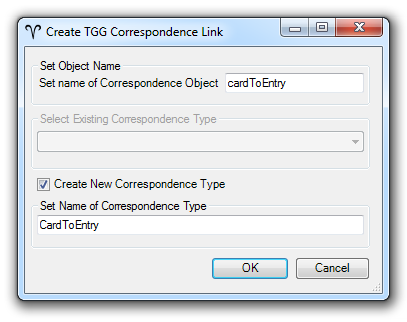
\includegraphics[width=0.7\textwidth]{ea_createNewCorrespondenceType}
  \caption{Create a new correspondence type on-the-fly}
  \label{ea:newCorrespondenceDialogue}
\end{center}
\end{figure}

\item[$\blacktriangleright$] Your diagram should now resemble Fig.~\ref{ea:cardtoentry_1}. We're not done yet though -- we still need to handle attributes!

\end{enumerate}

We must create a series of constraints in order to specify how relevant attributes should be handled. Let's first define a construct for every
\texttt{entry\-.cont\-ent}, \texttt{card.back}, and \texttt{card.face} EString values so that it's easy to (temporarily) persist the values during the
transformation. This will help us figure out how we should combine the front and back of each \texttt{card} as a single \texttt{content} attribute and,
in the opposite direction, help to separate the contents so that they may be split into \texttt{card.back} and \texttt{card.face}.

Let's define \texttt{entry\-.cont\-ent} as: \texttt{<word>:<mean\-ing>}. \texttt{card\-.back} should therefore be \texttt{Quest\-ion:<word>} and
similarly, \texttt{card\-.face} should be \texttt{Ans\-wer:<mean\-ing>}. 

\newpage

  \begin{figure}[htbp]
  \begin{center}
    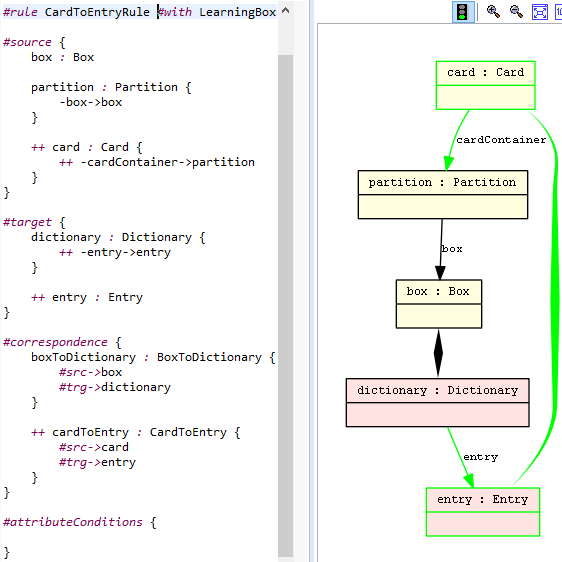
\includegraphics[width=\textwidth]{ea_cardToEntryRule}
    \caption{\texttt{CardToEntryRule} without attribute manipulation}
    \label{ea:cardtoentry_1}
  \end{center}
  \end{figure}


\begin{itemize}

\item[$\blacktriangleright$] We can now define three \emph{attribute constraints} to implement this. Luckily, we have two predefined constraints,
\texttt{addPrefix} and \texttt{concat} to help us. Use the toolbox again to create a new TGG constraint, and add the following to your diagram:

  \item \verb|addPrefix("Question", word, card.back)|  
  
  \item \verb|addPrefix("Answer", meaning, card.face)|
  
  \item \verb|concat(":", word, meaning, entry.content)|

\end{itemize}

Your rule should now resemble Fig.~\ref{ea:cardtoentry_2}, where ``Question'' and ``Answer'' are EString literals, \texttt{word} and \texttt{meaning} are
temporary variables, and \texttt{card.face}, \texttt{card.back}, and \texttt{entry.content} are attribute expressions (this should be familiar from SDM story
patterns).

\begin{figure}[htbp]
\begin{center}
  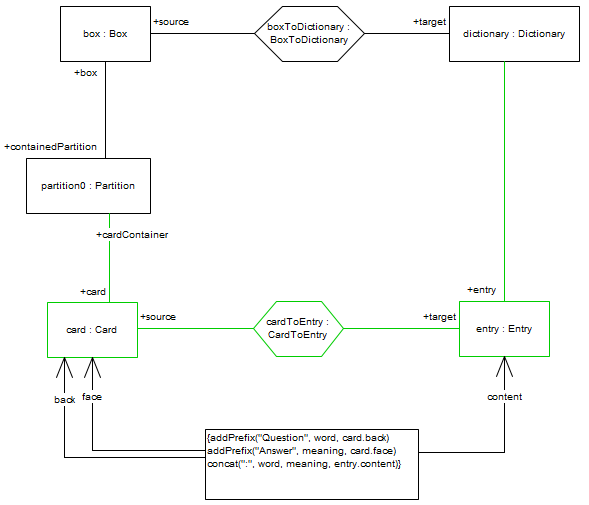
\includegraphics[width=\textwidth]{ea_CardToEntryRuleFirstConstraints}
  \caption{Attribute manipulation for \texttt{card} and \texttt{entry}}
  \label{ea:cardtoentry_2}
\end{center}
\end{figure}
\FloatBarrier

Our final task is to specify where a new \texttt{card} (when transformed from an \texttt{entry}) will be placed.  We purposefully created three
partitions to match the three difficulty levels, but if you check the constraints drop-down menu, there is nothing that can implement this specific kind of
mapping. We will therefore need to create our own constraint to handle this.

\begin{enumerate}

\item[$\blacktriangleright$] Add one more constraint to your diagram but, instead of choosing a predefined constraint, click ``Add'' just below the
drop-down menu to create a custom one. Name it \texttt{IndexToLevel}, and enter the values given in Fig. \ref{ea:create_new_constraint}.

\begin{figure}[htbp]
\begin{center}
  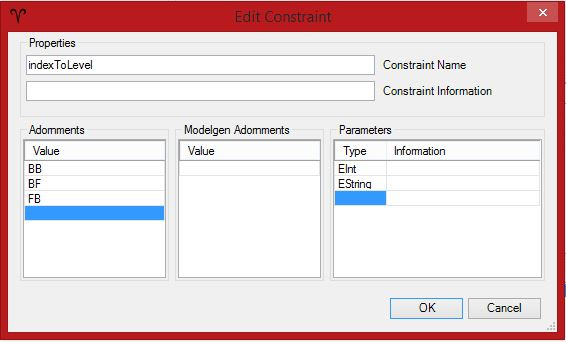
\includegraphics[width=0.9\textwidth]{ea_uniqueConstraint}
  \caption{Creating an unique constraint}
  \label{ea:create_new_constraint}
\end{center}
\end{figure}
\FloatBarrier

\item[$\blacktriangleright$] Please note that this is just a specification of a custom constraint -- we still need to implement in Java! Since we're so close to
finishing this TGG rule however, let's finish and export what we've made to Eclipse before doing so. We'll explain the exact meaning of the mysterious
adornments and parameters of the constraint in a moment. For now, just make sure you enter the exact values in Fig.~\ref{ea:create_new_constraint}. 

\item[$\blacktriangleright$] Save the new constraint, then select it from the drop-down menu in the TGG Constraint Dialog. Enter \texttt{partition0.index} as an
\texttt{EInt} value, and \texttt{entry.level} as an \texttt{EString}.

\item[$\blacktriangleright$] Your completed TGG rule should resemble Fig.~\ref{ea:cardtoentry_complete}. Great work! All that's left to do is implement the
\texttt{IndexToLevel} constraint, and give your transformation a test run.

\item[$\blacktriangleright$] Check out Fig.~\ref{eclipse:allReferences} in Section 4.3 to see how \texttt{BoxToDictionaryRule} is specified in the textual
syntax, or Fig.~\ref{eclipse:c2eDone} in Section 4.4 for the \texttt{CardToEntryRule}.

\end{enumerate}

\newpage

\vspace*{3cm}

\begin{figure}[htbp]
\hspace{-2cm}
  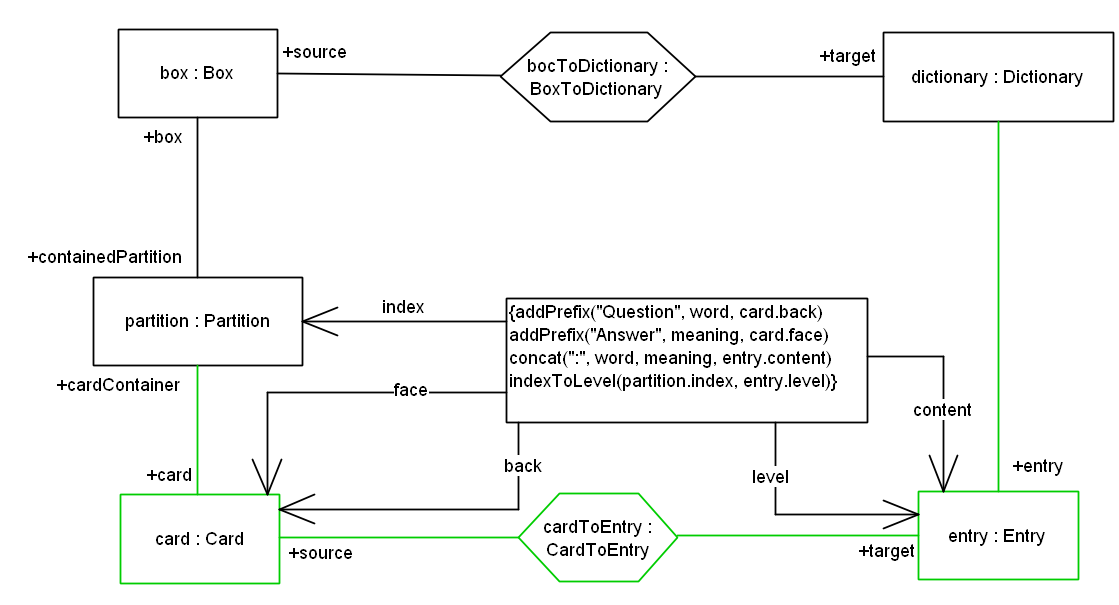
\includegraphics[width=1.2\textwidth]{ea_CardToEntryRuleComplete}
  \caption{\texttt{CardToEntryRule} with complete attribute manipulation}
  \label{ea:cardtoentry_complete}
\end{figure}

\jumpSingle{subsec:IndexToLevel}
